\chapter{Dinámica de Fluidos}

\begin{miparrafo}
La reología (palabra introducida por Eugene Bingham en 1929) es la rama de la física de medios continuos que se dedica al estudio de la deformación y el fluir de la materia.

La hidrodinámica o dinámica de fluidos es la rama de la reología que estudia la dinámica de los fluidos (gases y líquidos en movimiento).

Para el estudio de la hidrodinámica se pueden considerar diferentes aproximaciones, dependiendo del problema que se vaya a abordar, como por ejemplo las siguientes: 

\begin{itemize}
\item En muchos casos, los cambios de densidad en los fluidos se pueden despreciar, por lo que se puede considerar que el fluido a estudiar es un líquido incompresible, es decir, que su densidad no varía con el cambio de presión. Por esta misma razón, dicha aproximación no se suele utilizar para modelar gases.
\item En algunos casos (en bastantes casos macroscópicos o en hidrodinámica cuántica) se considera despreciable la pérdida de energía por la viscosidad, ya que la pérdida de energía debido a esta es mucho menor que la debida a la inercia de su movimiento.
\item En muchos casos, se puede suponer que el flujo de los líquidos alcanza un régimen estable denominado régimen estacionario, en el que la velocidad del líquido en cualquier punto es independiente del tiempo.
\end{itemize}
La hidrodinámica tiene aplicaciones en múltiples escalas que van desde la escala nanoscópica a la macroscópica.
 
Daniel Bernoulli fue uno de los primeros matemáticos que realizó estudios de hidrodinámica, siendo precisamente él quien dio nombre a esta rama de la física con su obra de 1738, Hydrodynamica.	
\end{miparrafo}

\section{Introducción}
El \emph{campo de velocidades} es el valor que toman las velocidades instantáneas de cada una de las partículas que componen en fluido. 

Como la velocidad es tangente en todo momento a la trayectoria, definiremos las \emph{líneas de corriente o currentilíneas} como las líneas tangentes a los vectores velocidad de las partículas del fluido en un instante determinado. En el caso más general son función del tiempo, el campo de velocidades y, por tanto, las currentilíneas varían con el tiempo.

Las líneas de corriente son funciones instantáneas del campo de velocidades.

\begin{figure}[H]
	\centering
	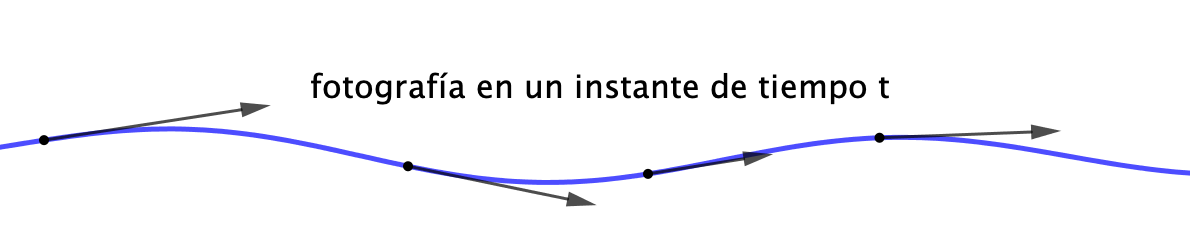
\includegraphics[width=1\textwidth]{imagenes/imagenes18/T18IM01.png}
	\end{figure}

Llamaremos \emph{línea de movimiento} de cada una de las partículas del fluido a la trayectoria real de estas.

Las líneas de corriente coincidirán con las líneas de movimiento cuando ambas sean constantes en el tiempo, lo que llamaremos \emph{régimen estacionario}.

En régimen estacionario, aplicaremos una causa externa que modificará el campo de velocidades y hará que las líneas de movimiento no coincidan con las líneas de corriente.

\section{Ecuaciones fundamentales de la hidrodinámica}

\begin{multicols}{2}
Elemento de volumen: $\dd \tau=\dd x \dd y \dd z$

en un instante, $ma=F$

Existen presiones y hay un campo exterior.

$\dd \vec F=\dd \vec f_e+\dd \vec f$, donde

$\vec F$ es la fuerza total, $\vec f_e$ la fuerza exterior y $\vec f$ la fuerza debida a las presiones del resto del fluido.
\begin{figure}[H]
	\centering
	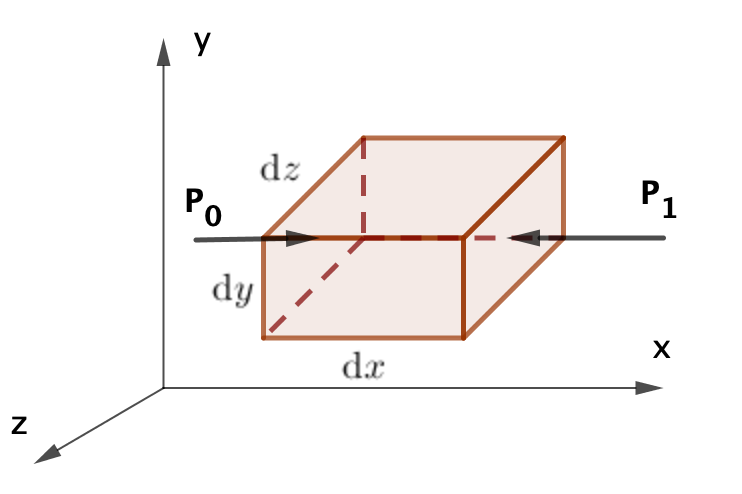
\includegraphics[width=.55\textwidth]{imagenes/imagenes18/T18IM02.png}
	\end{figure}	
\end{multicols}

$\dd \vec f_e=\vec a_e \dd m=\vec a_e \rho \dd \tau$; $\ \rho$, densidad del fluido.

$P=P(x,y,z),\qquad \dd f_x=(P_o-P_1=\dd y \dd z$

$\displaystyle \dd P=\pdv{P}{x}\dd x+\pdv{P}{y}\dd y++\pdv{P}{z}\dd z$

Considerando que la presión aumenta a lo largo del eje $X$,

$\dd f_x=\displaystyle - \pdv{P}{x}\dd x \ \dd y \dd z= -\pdv{P}{x} \dd \tau$

Análogamente, $\displaystyle \dd f_y=-\pdv{P}{y} \dd \tau;\qquad \dd f_z=-\pdv{P}{z} \dd \tau$

Luego $\displaystyle \dd \vec f= -\left(\vec i \pdv{P}{x}+\vec j \pdv{P}{y}+\vec k \pdv{P}{z} \right) = -\overrightarrow{\grad}P \ \dd \tau$

Finalmente:  $\displaystyle \vec a \rho \dd \tau = \vec a_E \rho \dd \tau -\overrightarrow{\grad}P \dd \tau$, de donde:

\begin{equation}
\label{ec.fdtal.hidrodinamica}
\subrayado{\ \boxed{ \  \boldsymbol{ \vec a = \vec a_e - \dfrac 1 \rho \overrightarrow{\grad}P	}\ } \ } \qquad \textbf{Ec. fdtal. hidrodinámica}
\end{equation}

Vamos ahora a deducir la otra ecuación fundamental de la dinámica, es consecuencia del teorema de conservación de la masa: \emph{ecuación de continuidad.}

\begin{miparrafodestacado}
``En todo elemento de volumen de un fluido en que no haya manantiales ni sumideros, la disminución experimental de la cantidad de fluido que sale por unidad de tiempo por una superficie cerrada, ha de ser igual a la disminución experimentada, en el mismo tiempo, por la masa de fluido contenida en el volumen limitado por dicha superficie''.	

El flujo de masa que pasa a través de una superficie cerrada S debe ser igual a la disminución, por unidad de tiempo, de la masa de fluido contenido en su interior.
\end{miparrafodestacado}

\textcolor{gris}{La ecuación de continuidad es una ecuación que nos explica que la cantidad de fluido que entra por medio de un tubo y que por lo general se mide en litros/segundo es es la misma que la cantidad de flujo que sale del mismo tubo, sin importar si el tuvo tiene más o menos radio a lo largo del mismo.}

\textcolor{gris}{Cuando el tubo por donde pasa el agua se encuentra en las debidas condiciones, lo que quiere decir que no tiene agujeros, la cantidad de agua que entra por segundo al no haber pérdidas debe de ser la misma cantidad que el agua que sale por segundo.}

\begin{multicols}{2}
$\displaystyle \rho \ \vec v=\dfrac {\dd m}{\dd \tau} \ \dv{\vec l}{t}= \dfrac {\dd m}{\dd S' \ \dd l} \ \dv{l}{t} \ \vec u_v \ \to $ 

$\boldsymbol{\rho \ \vec v = \dfrac{\dd m}{\dd S' \ \dd t} \ \vec u_v}$

Esto es la cantidad de fluido que pasa por unidad de tiempo y de elemento de área.

\begin{figure}[H]
	\centering
	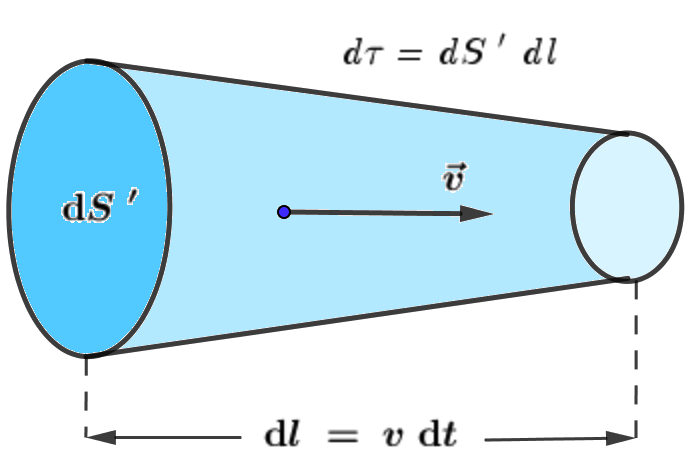
\includegraphics[width=.5\textwidth]{imagenes/imagenes18/T18IM03.png}
	\end{figure}
\end{multicols}
\vspace{30mm} %***************************************************
\begin{multicols}{2}
$\rho \vec v \cdot  \dd \vec S=\rho v \dd S \cos \varphi=$

$=\dfrac {\dd m}{\dd S'\ \dd t} \dd S \cos \varphi=$

$=\dfrac{\dd m}{\dd S \cos \varphi \dd t}\dd S \cos \varphi=\dfrac {\dd m}{\dd t}$
\begin{figure}[H]
	\centering
	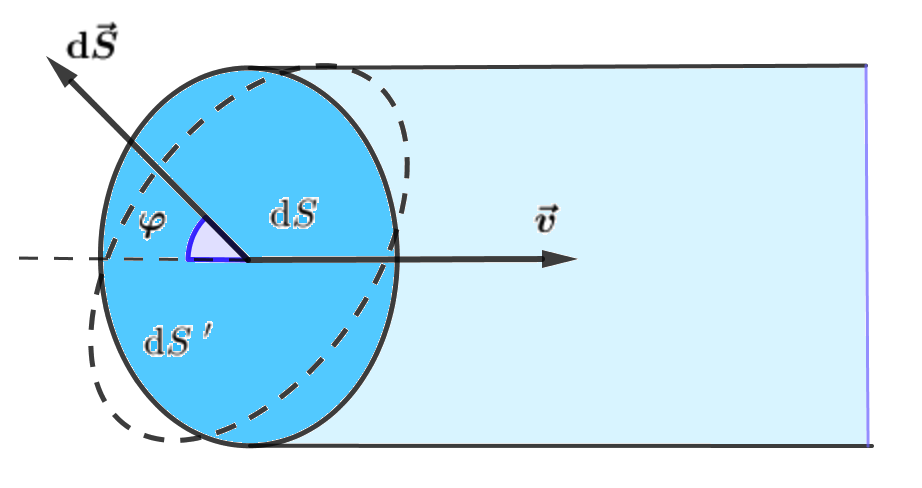
\includegraphics[width=.5\textwidth]{imagenes/imagenes18/T18IM04.png}
	\end{figure}
\end{multicols}



\begin{multicols}{2}
$\quad$

Cogeremos la cantidad de fluido que en un tiempo $t$ entra en la superficie $EFGH$ y le restaremos el que sale por $ABCE$. Obtendremos así la variación neta de masa en el eje $X$
\begin{figure}[H]
	\centering
	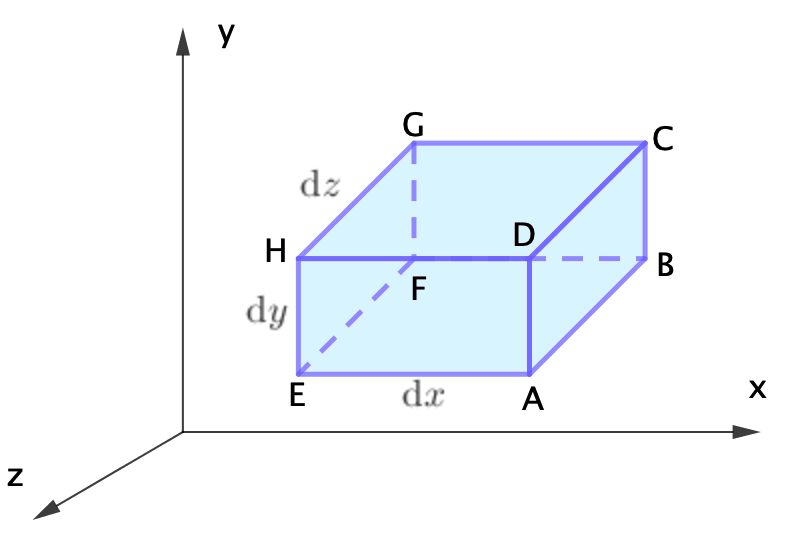
\includegraphics[width=.5\textwidth]{imagenes/imagenes18/T18IM05.png}
	\end{figure}
\end{multicols}

Dirección eje x: 

Supongamos que tenemos $\rho, \ \vec v$ en la cara $EFGH$ y $\rho+\dd \rho,\ \vec v+\dd \vec v$ en la cara $ABCD$.

------ En la cara $ABCD$

$\displaystyle \rho + \dd \rho=\rho +\dv{\rho}{x}\dd x+\dv{\rho}{y}\dd y+\dv{\rho}{z}\dd z$

$\displaystyle \vec v + \dd \vec v= \vec v + \dv{\vec v}{x}\dd x+\dv{\vec v}{y}\dd y+\dv{\vec v}{z}\dd z$

De izquierda a derecha, a lo largo del eje $X$, las magnitudes no varían con $y$ no con $z$: $\ \dd y=\dd z=0$

$\displaystyle (\rho+\dd \rho) (\vec v+\dd \vec v)\ \dd y \ \dd z \ \vec i=
\left(\rho+\dv{\rho}{x} \dd x \right) \left(\vec v+\dv{\vec v}{x}\dd x \right)\ \dd y \ \dd z \ \vec i=$

$=\displaystyle \rho v_x \dd y \dd z+\rho \pdv{v_x}{x} \dd x \dd y \dd z + \pdv{\rho}{x}v_x \dd x \dd y \dd z + \rho \dv{v_x}{x} \cancelto{0}{\dd^2 x} \dd y \dd z $

------ En la cara $EFGH: \qquad \rho \vec v \cdot (-\vec i) \ \dd y \dd z=-\rho v_x \dd y \dd z$

Sumando estas dos expresiones, obtendremos la variación de masa total a lo largo del eje $X$ que estamos buscando.

$\displaystyle \rho \pdv{v_x}{x} \dd x \dd y \dd z + \pdv{\rho}{x}v_x \dd x \dd y \dd z  =\pdv{\rho\ v_x}{x} \dd x \dd y \dd z=\pdv{(\rho v_x)}{x} \dd \tau$

Lo mismo ocurre en los ejes $\displaystyle Y,\ Z:\qquad \pdv{(\rho v_y)}{y} \dd \tau; \quad \pdv{(\rho v_z)}{z} \dd \tau$

En consecuencia, la variación de masa será:

$\displaystyle \left[ \pdv{(\rho v_x)}{x} +\pdv{(\rho v_y)}{y}+\pdv{(\rho v_z)}{z} \right] \ \dd \tau = \overrightarrow{\grad} \cdot (\rho \vec v) \ \dd \tau$. \textcolor{gris}{\small{$\quad (\overrightarrow{\grad}\cdot\ $} es la divergencia\normalsize{.})}

\vspace{5mm} %**********************************************
\rule{5cm}{0.2pt}

\textcolor{gris}{
\underline{Divergencia}:}

\textcolor{gris}{$\displaystyle \overrightarrow{\grad}\cdot \vec A=\left( \vec i \pdv{x}+\vec j \pdv{y}+\vec k \pdv{z} \right) \cdot \left( \vec i A_x+\vec j A_y+\vec k A_z \right) = \pdv{A_x}{x}+\pdv{A_y}{y}+\pdv{Az}{z} $}

\rule{5cm}{0.2pt}
\vspace{5mm} %**********************************************

Como el volumen no depende del tiempo, $\displaystyle -\dv{m}{t}=-\dv{\rho \dd \tau}{t}=-\dd \tau \pdv{\rho}{t}$ 

\textcolor{gris}{Tomamos derivadas parciales en vez de normales pues $\rho$ depende de más variables, $\rho=\rho(x,y,z,)$.}

$\displaystyle \dd \tau \left( \overrightarrow{\grad} \cdot (\rho \vec v) \right) = - \dd \tau \pdv{\rho}{t}$, por lo que:

\begin{equation}
\label{ecc.continuidad}
\subrayado{\ \boxed{ \ \boldsymbol{ \overrightarrow{\grad}\cdot (\rho \vec v) \ = \ -\pdv{\rho}{t} }  \ }  \ }	 \qquad \textbf{Ecuación de continuidad}
\end{equation}

\vspace{5mm} %**********************************************
Un caso particular es el de 

\hspace{10mm} \textbf{fluidos incompresibles}: $\rho=cte \to \overrightarrow{\grad}\cdot (\vec v) \ = \ 0$

Este tipo de fluidos recibe el nombre de \textbf{\emph{fluidos soleniodales}} pues la divergencia de su velocidad es cero. En fluidos solenoidales las líneas de corriente se cierran sobre sí mismas, es decir, la cantidad de fluido que entra en cualquier superficie cerrada es igual a la que sale de ella (en cualquier superficie cerrada entran tantas líneas como salen de ella.)
\begin{multicols}{2}
$\rho=cte \to \overrightarrow{\grad}\vec v=0$

$S_1=A_1$ y $S_2=A_2$ son dos superficies transversales al tubo de corriente.

En general, $\dd m=\rho \dd \tau=\rho S v \dd t$

$\rho=cte \to \dd m_1=\dd m_2$

Luego: $S_1v_1=S_2v_2$

Es decir, $\subrayado{\ \boldsymbol{\boxed{Sv=cte}} \ }$

que es otra forma de escribir la \textbf{ecuación de continuidad para fluidos con} $\boldsymbol{\rho=cte}$. Es la que aparece en libros elementales.
\begin{figure}[H]
	\centering
	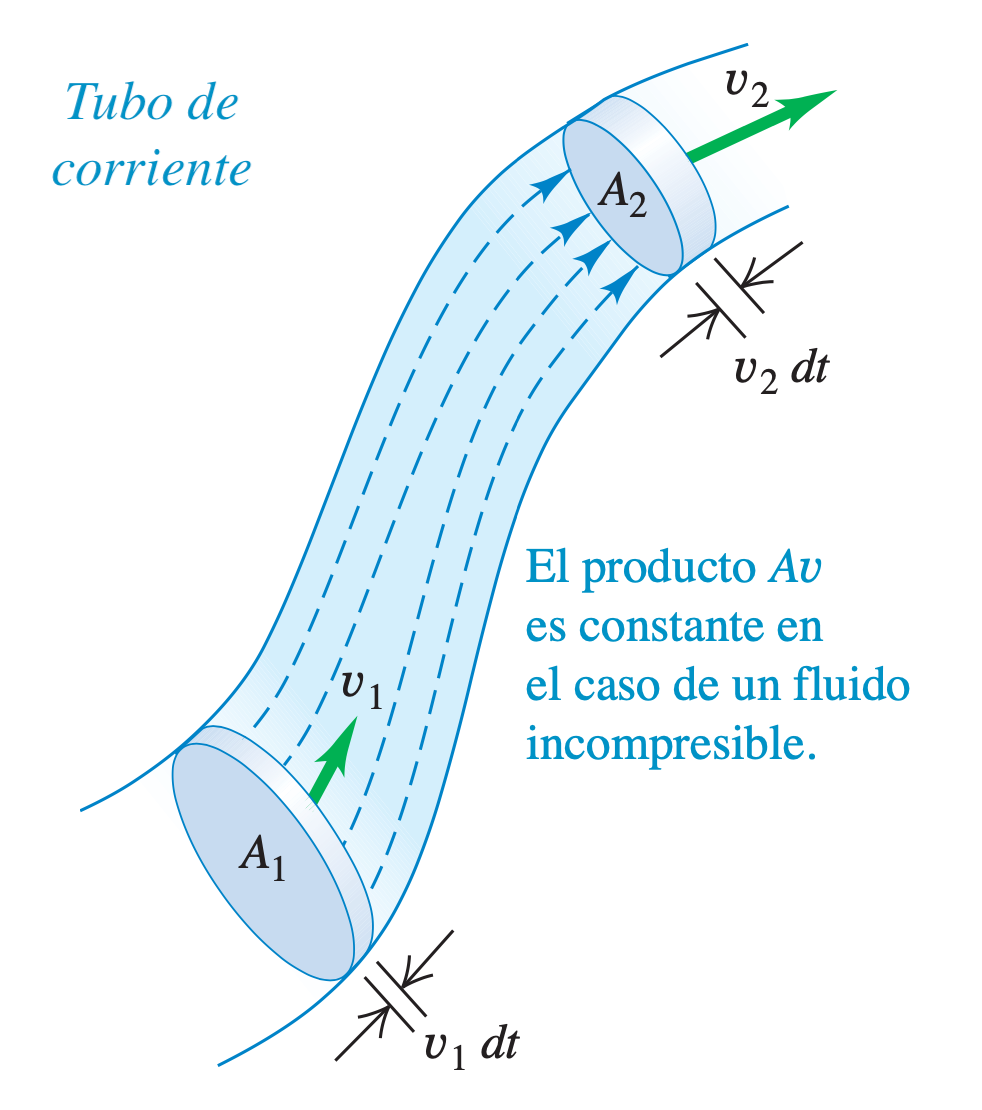
\includegraphics[width=.55\textwidth]{imagenes/imagenes18/T18IM06.png}
	\end{figure}	
\end{multicols}

\section{Ecuación de Bernoulli}

Suponemos que el campo exterior de fuerzas es el campo gravitatorio.

$\vec a_e=\vec g=-g \ \vec k=-g \ \overrightarrow{\grad}_z$

La ecuación fundamental de la hidrodinámica (\ref{ec.fdtal.hidrodinamica}) es, ahora,

$\vec a = -g \ \overrightarrow{\grad}_z - \dfrac 1 \rho \overrightarrow{\grad}P$, multiplicando escalarmente por el elemento de línea de corriente $\dd \vec l$

$\vec a \cdot \dd \vec l= -g \ \overrightarrow{\grad}_z \cdot \dd \vec l- \dfrac 1 \rho \overrightarrow{\grad}P \cdot \dd \vec l$

$\vec a \cdot \dd \vec l=a \dd l \cos \varphi =a_t \dd l$, componente tangencial de la aceleración.

$\displaystyle a_t \dd l=\dv{v}{t}\dd l = \dv{v}{t} v \dd t = \dfrac 1 2 \dd v^2$

Como, $\displaystyle \overrightarrow{\grad}\phi \cdot \dd \vec \phi =\left( \vec i \pdv{\phi}{x}+\vec j \pdv{\phi}{y}+\vec k \pdv{\phi}{z} \right) \cdot \left( \vec i \dd x + \vec j \dd y + \vec k \dd z \right)= $

$=\displaystyle \left(  \pdv{\phi}{x} \dd x +  \pdv{\phi}{y} \dd y +  \pdv{\phi}{z} \dd z
 \right) = \dd \phi$
 
 tendremos que  $\ \overrightarrow{\grad}_z\cdot \dd l=\dd z ;\qquad \overrightarrow{\grad}P \cdot \dd l=\dd P$

Luego, $\ \dfrac 1 2 \dd v^2 = -g \dd z -\dfrac 1 \rho \dd P$; multiplicando por $\rho$,

\begin{equation}
\subrayado{ \ \boxed{ \ \boldsymbol{
\dd P \ +\ \dfrac 1 2 \ \rho \ \dd v^2 \ +\  g\ \rho \ \dd z \ =\  0	 \qquad \textbf{Th. Bernoulli} 
} \ } \ }
\end{equation}

Los tres términos de la ecuación de Bernoulli son: la presión debida al fluido, la presión cinética y la presión debida a la altura; en ese orden.

\underline{Observación}: La hidrostática es la parte de la hidrodinámica en que $v=0 \to \dd P + g \rho \dd z=0$, que es la ecuación fundamental de la hidrostática.  (ec. \ref{ec.fdtal.hidrostatica})

Para fluidos incompresibles, $\rho=0$ la ecuación de Bernoulli se reduce a la que aparece en libros elementales:

$\rho =cte \to \dd \left( P+\dfrac 1 2 \rho v^2+\rho g z \right) =0 \to P+\dfrac 1 2 \rho v^2+\rho g z =cte$

$$\subrayado{ \boldsymbol{\ P_1+\dfrac 1 2 \rho v_1^2+\rho g z_1 =P_2+\dfrac 1 2 \rho v_2^2+\rho g z_2} \ }$$

\begin{figure}[H]
	\centering
	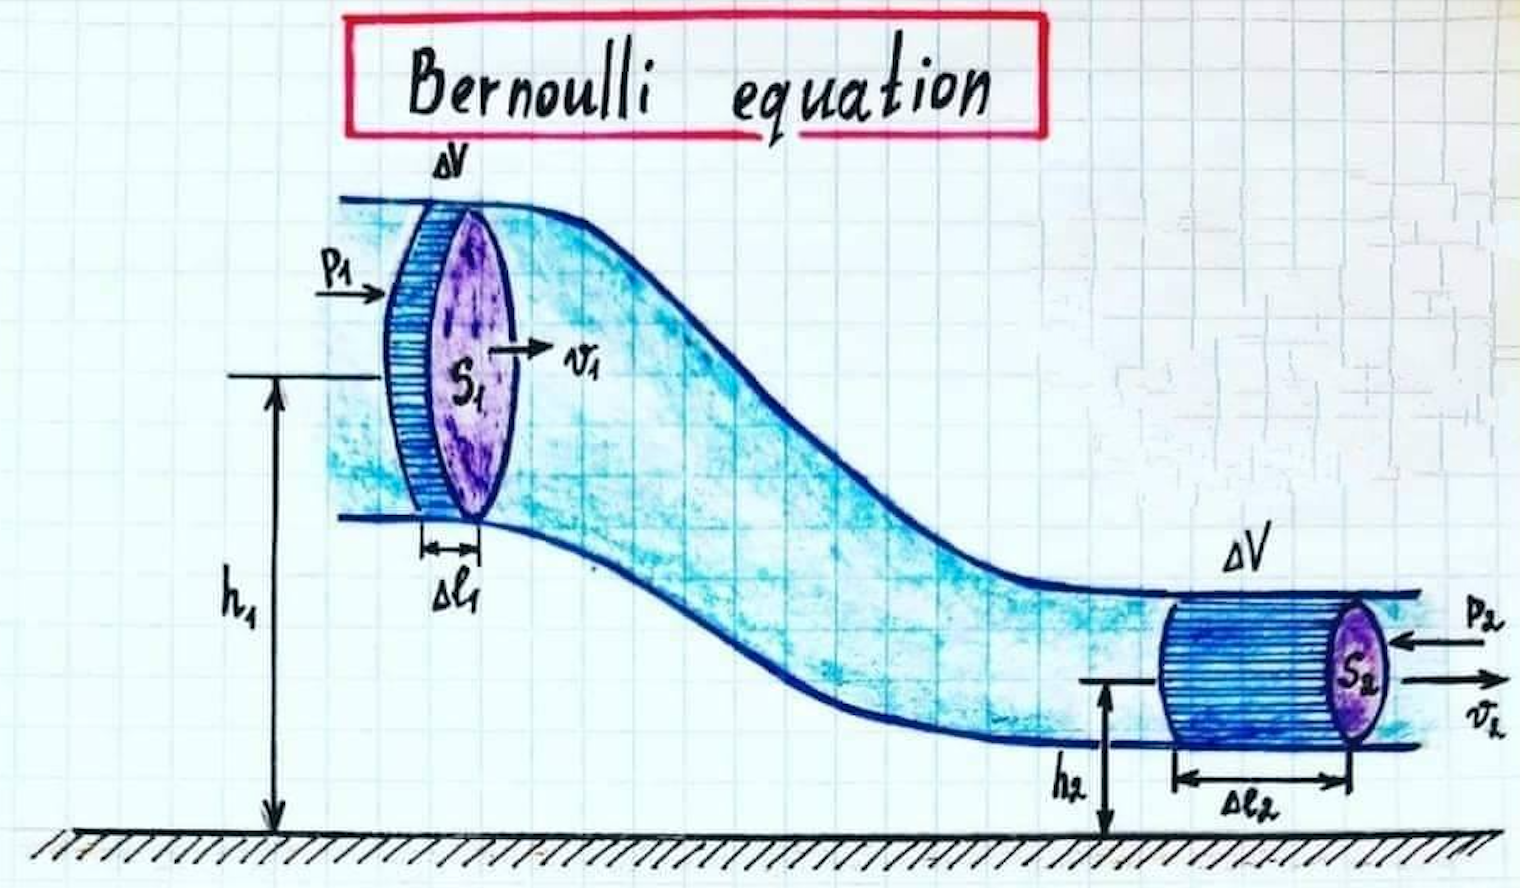
\includegraphics[width=1\textwidth]{imagenes/imagenes18/T18IM07.png}
	\end{figure}	

\subsection{Aplicaciones del teorema de Bernoulli: Teorema de Torricelli y Efecto Venturi}

\vspace{10mm} %*************************************

\textbf{\large{Teorema de Toricelli}}\normalsize{.}

\begin{miparrafodestacado}
	Como consecuencia del Th. de Bernuilli, el Th. de Torricelli resuelve la cálculo de la velocidad con que emerge un fluido de un recipiente al que se la ha practicado un agujero.
\end{miparrafodestacado}


\begin{multicols}{2}
$\rho = cte$; campo gravitatorio.

$P_1+\dfrac 1 2 \rho v_1^2 +\rho g y_1=$

$=P_2+\dfrac 1 2 \rho v_2^2 +\rho g y_2$

$y_2-y_1=h; \ P_1=P_o; \ P_2=P$, 

$v_1^2=v_2^2+2\dfrac{P-P_0}{\rho}+2gh$

\underline{$1^a$ hipótesis}: presión atmosférica, depósito abierto.

$v_1^2=v_2^2+2\cancel{\dfrac{P-P_0}{\rho}}+2gh =v_2^2+2gh$
\begin{figure}[H]
	\centering
	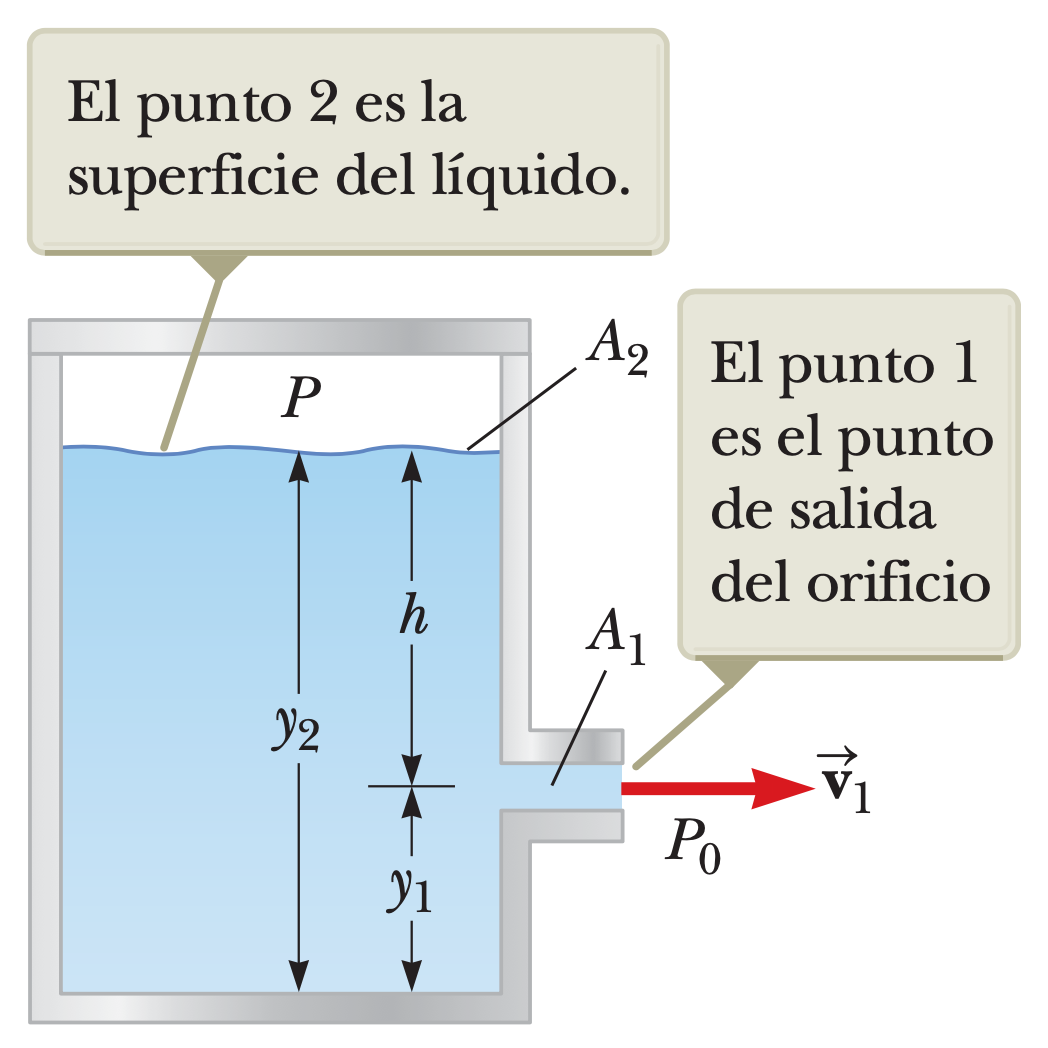
\includegraphics[width=.5\textwidth]{imagenes/imagenes18/T18IM08.png}
	\end{figure}	
\end{multicols}

Ecuación continuidad: $\quad S_1v_1=S_2v_2$

Observacionalmente, el líquido va a ser más estrecho que el agujero. Experimentalmente se encuentra que $S_1\approx 65\%$ de la superficie del orificio practicado para orificios circulares de borde fino. 

Como

 \underline{$2^a$ hipótesis}: $S_1<<S_2 \ \to \ v_1>>v_2 \ $Con lo que:
 
 \begin{equation}
 \boldsymbol{ v_1 \approx \sqrt{2gh}	 } \qquad  \textbf{Teorema de Torricelli}
 \end{equation}
 
\vspace{10mm} %*************************************
 
\textbf{\large{Efecto Venturi}}\normalsize{.}

\begin{miparrafodestacado}
``En aquellas conducciones en que disminuye la sección, la conducción del fluido aumenta la velocidad y disminuye la presión''.	
\end{miparrafodestacado}

\begin{multicols}{2}
$\rho = cte$; campo gravitatorio.

Como $y_1=y_2$

$P_1+\dfrac 1 2 \rho v_1^2 +\cancel{\rho g y_1}=$

$=P_2+\dfrac 1 2 \rho v_2^2 +\cancel{\rho g y_2}$

Ecuación continuidad: 

$S_1v_1=S_2v_2$
\begin{figure}[H]
	\centering
	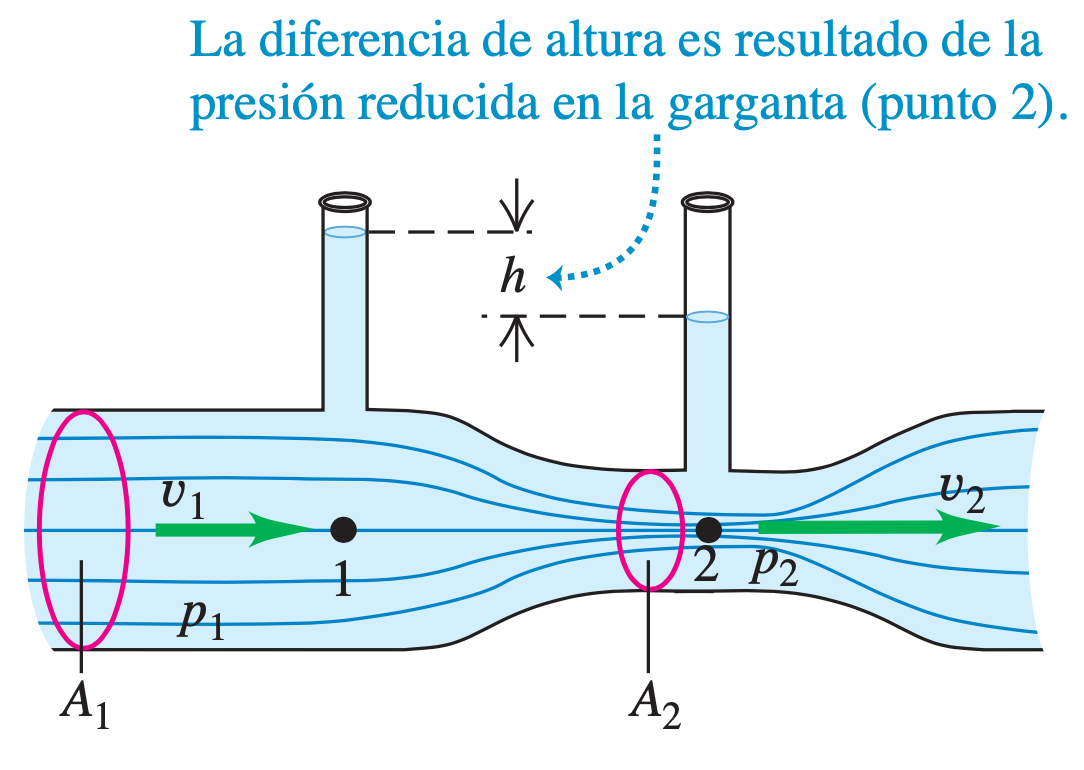
\includegraphics[width=.5\textwidth]{imagenes/imagenes18/T18IM09.png}
	\end{figure}	
\end{multicols}	
$v_2=v_1\ \dfrac{S_1}{S_2}; \quad S_1>S_2 \to v_2>v_1.\ $ 
Como 
$\ P_1+\dfrac 1 2 \rho v_1^2 =P_2+\dfrac 1 2 \rho v_2^2$

\begin{equation}
P_2\ <\ P_1 \qquad \text{Efecto Venturi}	
\end{equation}

$$ \subrayado{\ \boldsymbol{ S\downarrow \quad v\uparrow \quad P\downarrow \qquad \qquad  \qquad S\uparrow \quad v\downarrow \quad P\uparrow }\ } $$

\section{Viscosidad}

Los fluidos ideales son los que siguen la ecuación de Bernoulli pero en realidad las partículas del fluido interaccionan entre ellas dando como resultado un rozamiento. No todos los fluidos presentan las mismas interacciones de rozamiento. 

Llamamos \textbf{\emph{viscosidad}} a la resistencia que tienen ciertas sustancias a fluir, representaremos por $\boldsymbol{\eta}$ al \emph{coeficiente de viscosidad}, es característico de cada sustancia.

\begin{figure}[H]
	\centering
	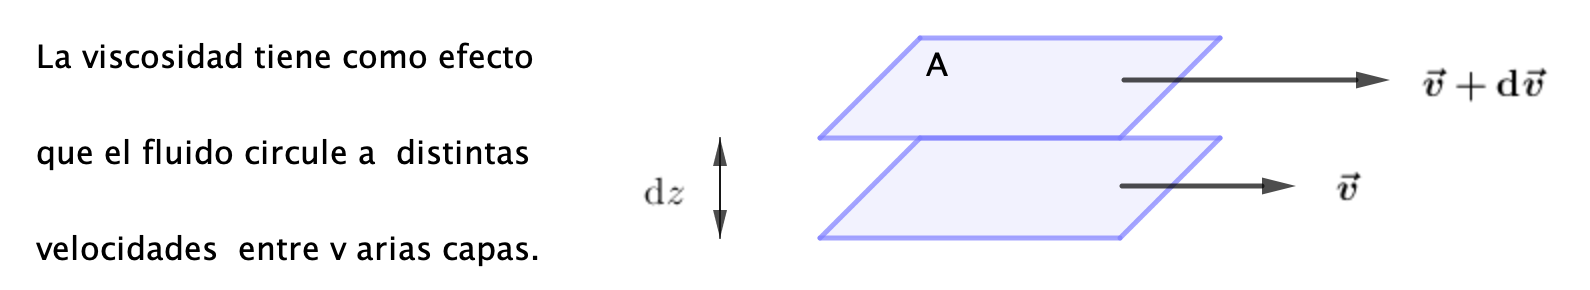
\includegraphics[width=1\textwidth]{imagenes/imagenes18/T18IM11.png}
	\end{figure}

\textbf{Hipótesis de Navier}: \emph{La fuerza entre las capas de fluido es proporcional a la superficie de las capas y al gradiente de velocidades, siendo la viscosidad la constante de proporcionalidad}

\begin{equation}
\label{Navier}
\subrayado{\ \boxed{\  \boldsymbol{F\ =\ \eta \ A \ \dv{v}{z}} \ } \ }	\qquad \text{Hipótesis de Navier}
\end{equation}

$\boldsymbol{\eta}$ es la fuerza tangencial que se ejerce sobre una superficie líquida de área unidad cuando, normalmente a la misma, existe un gradiente de velocidades igual a la unidad. $\quad [\eta]=ML^{-1}T^{-1}$.  Su unidad en el sistema $cgs$ es el $\mathrm{Poise},\ P$,  debido al fisiólogo francés Jean Léonard Marie Poiseuille (1799-1869) y en el $SI$ el $\mathrm{decaPoise}=10\ \mathrm{Poise}$.

Se llama \emph{viscosidad cinemática}, $\nu$ al cociente de la viscosidad entre la densidad: $\quad \nu=\dfrac{\eta}{\rho}$; $\quad [\ \nu \ ]=L^2 T^{-1}$, la unidad en el $cgs$ es el Stoke, del físico irlandés George Gabriel Stokes (1819-1903); $\ 1\mathrm{St}=1 \mathrm{cm}^2 \ \mathrm{s}^{-1}$.

En algunas sustancias $\eta=\eta(T)$, la viscosidad es función de la temperatura. Para el agua, a $18\ C$, $\eta_{_{H_2O}}=0.01056\ P$

\textbf{\large{Formula de Stokes}}\normalsize{.}

Estudió el efecto que se produce al depositar un cuerpo. en una masa fluida y observar la fuerza que la velocidad del fluido ejerce sobre el cuerpo. 

La ecuación de esta fuerza viscosa depende de la geometría del cuerpo. Para un cuerpo de simetría esférica:

$$F=6 \ \pi \ r \ \eta \ v$$

$r$ radio de la esfera, $\eta$ coeficiente de viscosidad del fluido, $v$ velocidad relativa del fluido respecto de la masa del fluido.

Las gotas de lluvia, al caer, son frenadas por esta fuerza que frena su caída; así, $\ F_{total}=F_{gravedad}-F_{empuje}-F_{Stokes}$, que hace que se alcance una \textbf{\emph{ velocidad límite }}.

$ma=mg-\rho_0gV-6\pi r\eta v \ \to \ \dfrac 4 3 \pi r^3 \rho a =\rho \dfrac 4 3 \pi r^3 g - \rho_o \dfrac 4 3 \pi r^3 g - 6 \pi r \eta v$

De donde se puede calcular la aceleración instantánea $a$.

Llegará un momento en que el empuje y la fuerza de Stokes igualen al peso, la aceleración será cero y la velocidad será constante, \emph{velocidad límite}, $v_L$

$\rho \dfrac 4 3 \pi r^3 g - \rho_o \dfrac 4 3 \pi r^3 g = 6 \pi r \eta v_L \to g 	\dfrac 2 9 r^2 (\rho - \rho_0)=\eta v_L$, y tendremos que

$$ \boldsymbol{v_L \ = \ \dfrac 2 9 \ \dfrac{g r^2 (\rho-\rho_0)}{\eta}} $$

\vspace{10mm} %*****************************************
\section{Régimen laminar y régimen turbulento}

Reynolds hizo notar que el flujo de un fluido por una conducción se realiza de distinto modo según la velocidad de éste sea pequeña o sea grande.

En 1883 Osborne Reynolds realizó su famoso experimento, que sirve para poner en evidencia las diferencias entre flujo laminar y turbulento. Este experimento consiste en inyectar colorante en el seno de un líquido que circula por un tubo largo de sección constante. Para velocidades pequeñas, Reynolds observo que este movimiento se caracteriza por ser permanente y por ser las líneas de corriente paralelas a las paredes del tubo. Bajo estas circunstancias el colorante forma una línea de corriente bien definida. Es el denominado \emph{movimiento laminar}. Sin embargo, si la velocidad del fluido se hace suficientemente grande, el movimiento fluido se hace muy sensible a cualquier perturbación y estas perturbaciones se amplifican rápidamente; el flujo se hace entonces muy irregular y pierde su carácter estacionario, se forman remolinos. Es el \emph{movimiento turbulento}. 

\begin{multicols}{2}
A pequeñas velocidades el líquido coloreado transcurre paralelamente a la conducción, pero al aumentar la velocidad, a partir de un valor crítico $v_c$, el líquido coloreado se enrolla en sí mismo y produce turbulencias hasta difuminarse en el fluido.

Para cada par líquido-conducción existe una $v_c$.
\begin{figure}[H]
	\centering
	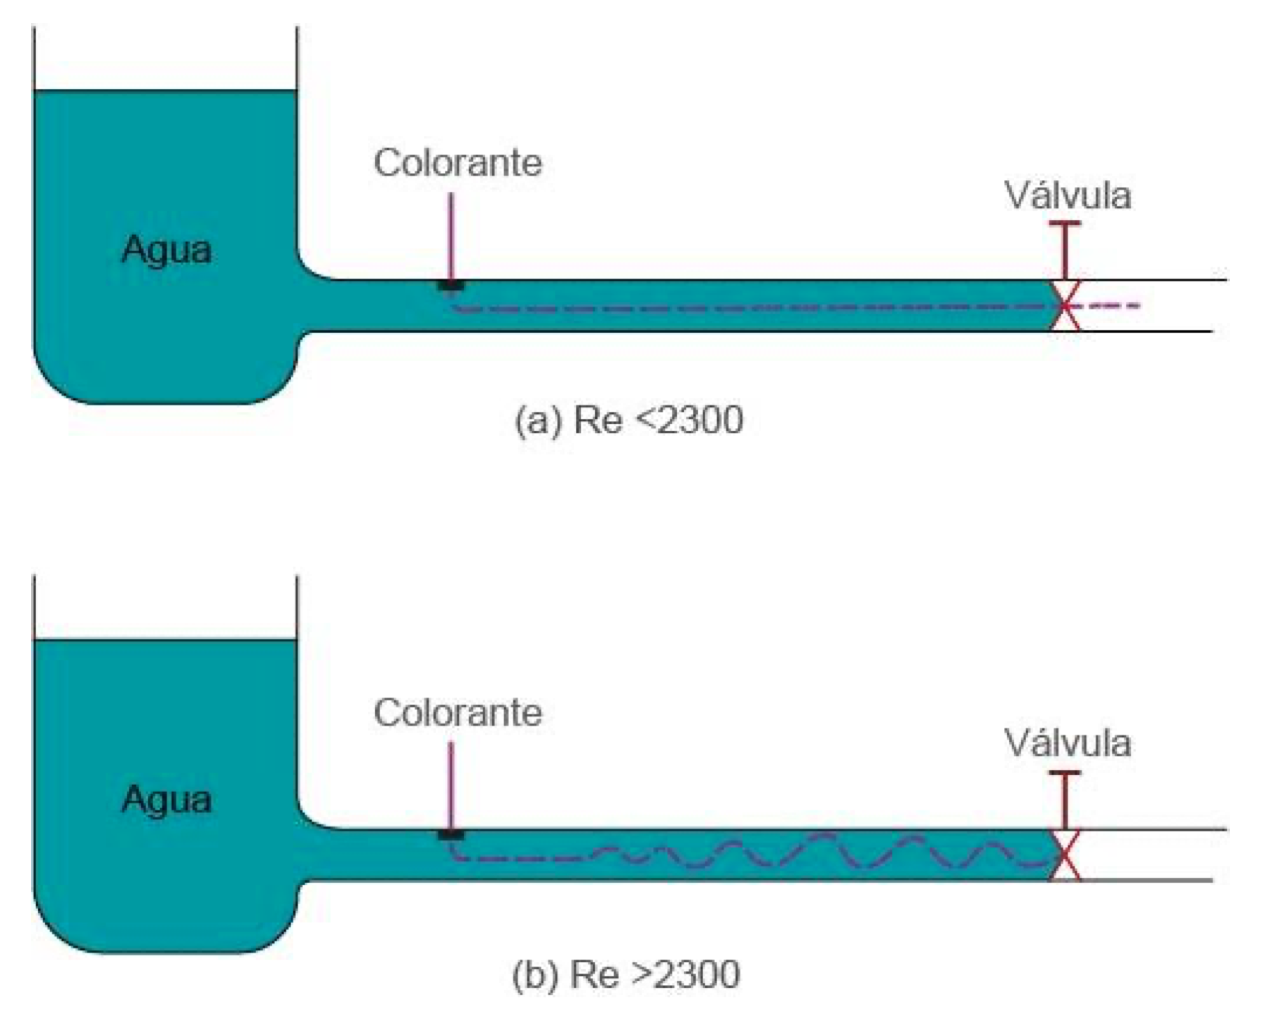
\includegraphics[width=.5\textwidth]{imagenes/imagenes18/T18IM12.png}
	\end{figure}
\end{multicols}


El \emph{número de Reynolds} es un coeficiente adimensional que nos indica si el régimen es laminar o turbulento para un fluido dado ($\eta,\ \rho$) en una conducción determinada (diámetro, $d$).

Llamando \emph{velocidad característica} del par fluido-conducción $v_0=\dfrac{\eta}{\rho d}$, Reynolds introduce su coeficiente adimensional $N_R=\dfrac {v}{v_0}$, así, 


$$N_R\ = \ \dfrac{v\ \rho \ d}{\eta} \ ; \qquad v\ = \ N_R\ v_0$$

Llamamos $\dfrac{v_c}{v_0}\ = \ N_{cR}\ \text{número de Reynolds crítico}$

Experimentalmente se encuentra que:

$$\begin{cases} \quad N_{cR}\ < \ 2400 & \to \ \text{régimen laminar}  \\  \quad N_{cR}\ > \ 2400 & \to \ \text{régimen turbulento}  \end{cases}$$

\textbf{Ejemplo}: \emph{Calcular la velocidad crítica del fluido-conducción, $v_0$, para $a)$ un tubo capilar de $0.1\ mathrm{mm}$ de diámetro y $b)$ otro de $d=1\ \mathrm{cm}$, ambos recorridos por agua.}

Trabajamos en el sistema cegesimal.

------ a) $\ v_0=\dfrac {\eta}{\rho \ d}=\dfrac{0.01056}{1\cdot 0.01}=1 \ \mathrm{cm\ s}^{-1}$

$v_c=N_{cR} \ \ v_0=2400 \times 1 =2400 \ \mathrm{cm\ s}^{-1}= 24 \ \mathrm{m\ s}^{-1}$, velocidad imposible de alcanzar en la práctica. 

Todos los tubos capilares con estas carateristicas son de régimen laminar.

------ b) $\ v_o=\dfrac{10^{-2}}{10\cdot 1}=10^{-3} \ \mathrm{cm\ s}^{-1}$

$v_c=N_{cR} \ \ v_0=2400 \times 1o^{-3} =2.4 \ \mathrm{cm\ s}^{-1}= 0.024 \ \mathrm{m\ s}^{-1}$ 

Dado a que esta velocidad es muy pequeña, normalmente en estos tubos habrá régimen turbulento.

\section{Fórmula de Poiseuille}

Consideramos un régimen laminar o de Poiseuille (fue lo que hizo Poiseuille al estudiar la circulación sanguínea).

Para régimen de Bernoulli encontramos $ P+\dfrac 1 2 \rho v^2 + \rho g h = cte$.

En régimen laminar hay rozamiento, existe una presión debido al rozamiento además de la presión debida a la masa del líquido $P$, de la presión cinética $\frac 1 2 \rho v^2$ y de la presión hidrostática  $\rho g h$.

$P_1+\dfrac 1 2 \rho v_1^2 + \rho g h_1=P_2+\dfrac 1 2 \rho v_2^2 + \rho g h_2 + \dfrac{\Delta Q}{\tau}$

Por el teorema de la conservación de la energía, La energía por unidad de volumen en una posición de la conducción es igual a la energía por unidad de volumen en otra posición más la energía disipada para que las lámina de fluido pase de la posición 1 a la 2. Esto supone una \emph{pérdida lineal de carga}, la presión disminuye linealmente a medida que se avanza en una conducción de régimen laminar.

Apliquemos esto a (1) una conducción horizontal de (2) la misma sección en toda ella:

$\mathrm{(1)}\ h_1=h_2;\quad  \mathrm{(2)}\ S_1=S_2 \ \to \ v_1=v_2 \quad P_1=P_2+ \dfrac{\Delta Q}{\tau}$

$$P_2 \ = P_1 \ - \ \dfrac{\Delta Q}{\tau}$$

ecuación que representa una recta siempre que $\dfrac{\Delta Q}{\tau}$ aumente linealmente a medida que se avanza en la conducción horizontal, como se comprueba experimentalmente.

\begin{figure}[H]
	\centering
	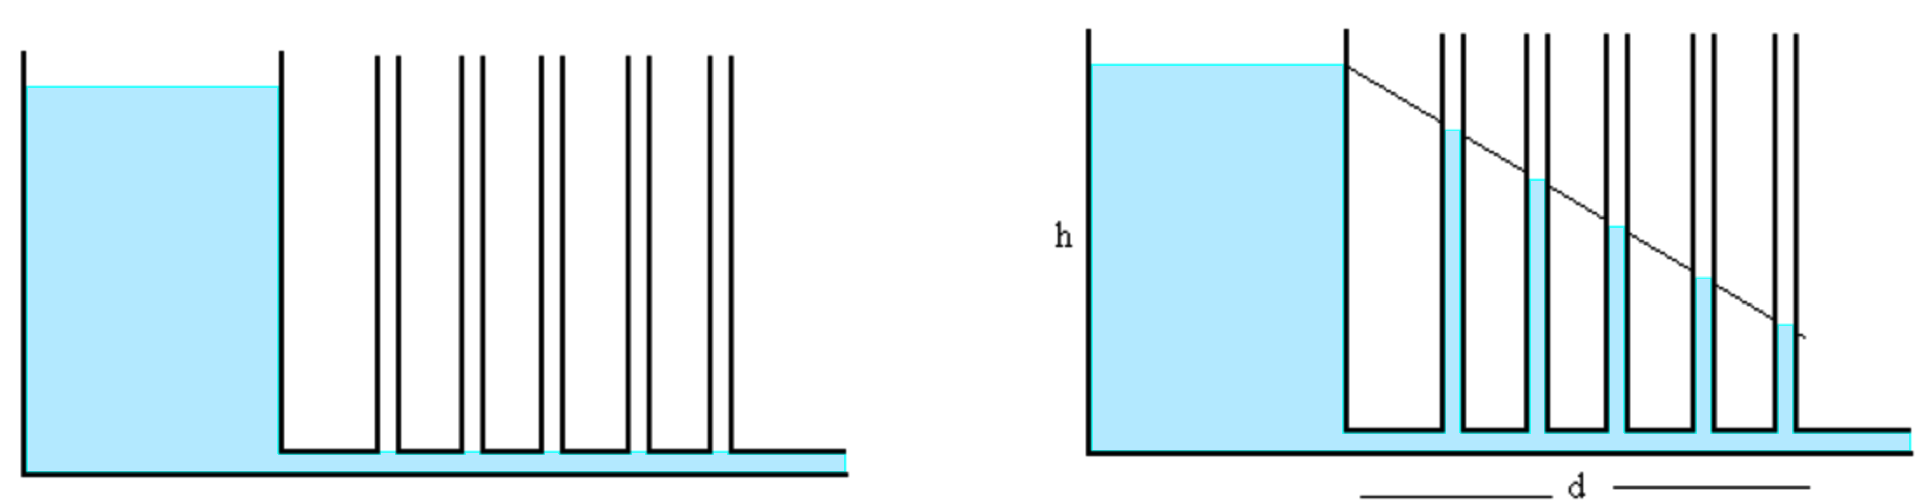
\includegraphics[width=.75\textwidth]{imagenes/imagenes18/T18IM13.png}
	\end{figure}

En un fluido ideal,  el líquido sale por la conducción con $v=\sqrt{2gh}$ de acuerdo con Torricelli. Toda la energía potencial se convierte en energía cinética. Con manómetros podemos comprobar que la presión en los tubos verticales es cero

En un fluido viscoso, el balance energético es diferente. Al abrir el extremo del tubo, sale fluido con una velocidad bastante más pequeña. Los tubos manométricos marcan alturas decrecientes, informándonos de las pérdidas de energía por rozamiento viscoso. En la salida, una parte de la energía potencial que tiene cualquier elemento de fluido al iniciar el movimiento se ha transformado íntegramente en calor. El hecho de que los manómetros marquen presiones sucesivamente decrecientes nos indica que la pérdida de energía en forma de calor es uniforme a lo largo del tubo. Es la llamada \emph{pérdida lineal de carga}.

\subsection{Gasto de una conducción en régimen laminar}

Se define \emph{\textbf{gasto}} como el volumen de líquido, por unidad de tiempo, que atraviesa una sección transversal de la conducción.

Vamos a determinar el gasto para una conducción cilíndrica de régimen laminar.

\begin{figure}[H]
	\centering
	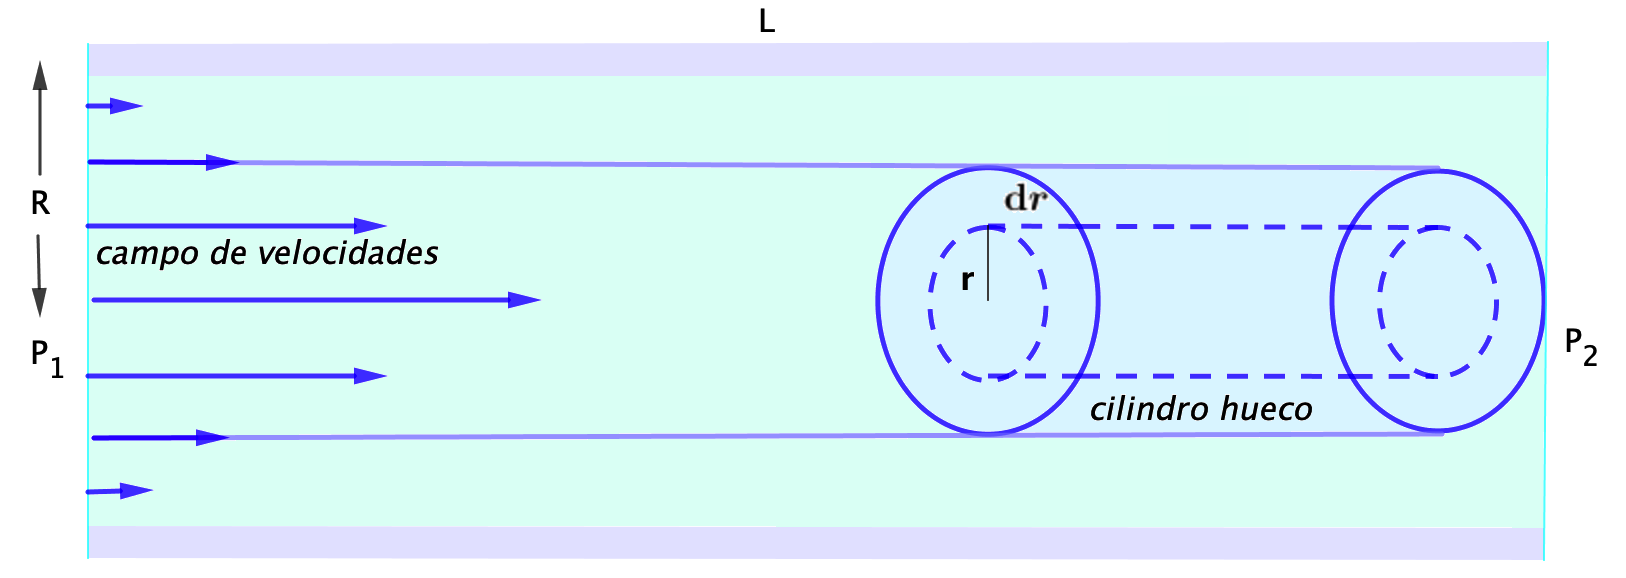
\includegraphics[width=1\textwidth]{imagenes/imagenes18/T18IM14.png}
	\end{figure}

Las partículas próximas al eje de la conducción sobre las partículas del cilindro hueco, por ser más veloces, ejercen una fuerza en el sentido de las velocidades. El fluido que circula más externamente en el cilindro hueco lo hace más despacio, ello conlleva una fuerza en sentido contrario. 

Matemáticamente, teniendo en cuenta la hipótesis de Navier (\ref{Navier}), tenemos:

$\displaystyle f_1=-\eta \ 2\pi r L \ \dv{v}{r}$

$\displaystyle f_2=+\eta \ 2\pi(r+\dd r)L \ \left( \dv{v}{r} + \dd \dv{v}{r} \right) = \eta \ L\ 2\pi (r+\dd r) \left( \dv{v}{r} +  \dv[2]{v}{r} \dd r \right)$

Además, debido a la diferencia de presiones,

$f_3=P_1\ 2\pi r \dd r -P_2\ 2\pi r \dd r= (P_1-P_2) \ 2 \pi r \dd r$

Por la ecuación de continuidad, $\dd (Sv)=0 \to S=cte \to v$, por un filete cualquiera de la conducción laminar es constante. Dimámicamente, la aceleración ha de ser cero $\to T_{total}=0 \to f_1+f_2+f_3=0$.

Luego, $\displaystyle \ (P_1-P_2)\ r + \eta L r \ \dv[2]{v}{r}+ \eta L \ \dv{v}{r}=0$

de otro modo, $\ \displaystyle (P_1-P_2) \ r + \eta \ L \ \dv{r} \left( r\ \dv{v}{r} \right) = 0$

separamos variables, $\ \displaystyle \dv{r} \left( r\ \dv{v}{r} \right) =-\dfrac{(P_1-P_2) \ r \ \dd r}{\eta \ L}$

integrando, $\ \displaystyle \cancel{r}\ \dv{v}{r} = -\dfrac{(P_1-P_2) }{2\ \eta \ L} \ r^{\cancel{2}} + \dfrac{\mathcal C}{r}$

Volviendo a separar variables, $\displaystyle \ \dd v = -\dfrac{(P_1-P_2) }{2\ \eta \ L} \ r \  \dd r  + \dfrac{\mathcal C}{r} \dd r$

integrando, $\displaystyle \ v=- \dfrac{(P_1-P_2) }{4\ \eta \ L} \ r^2 + \mathcal C \ \ln{r} + \mathcal B;\qquad \mathcal B, \mathcal C$ ctes. integración.

--- Para $r=0$, estamos en el eje de simetría de la conducción $\to v_{eje}=v_{max}$. Contradicción, $ \underset {r\to 0} {\mathrm{lim}}\ \mathrm{ln} r=-\infty \ \to \ v_-\infty$, no tiene sentido. Exigimos, para eliminar esta contradicción, que $\ \boldsymbol{\mathcal C=0}$

--- Para $r=R \to v=0 \to \mathcal B=\dfrac{P_1-P_2}{4\eta L}R^2$

de donde:

\begin{equation}
v \ = \ \dfrac{P_1-P_2}{4\pi \eta L}\ (R^2-r^2)	
\end{equation}

Nos interesa el \textbf{gasto}, volumen de líquido recorrido por unidad de tiempo y unidad de área. Los tubos cilíndricos más próximos al eje aportarán más fluido que los cilindros cercanos a la pared. Vamos a determinar el elemento de gasto con el que contribuyen esos cilindros elementales.

$\displaystyle \dd G=\dv{t} \dd \tau =\dv{t} \ ( L \cdot 2\pi r \dd r)=v\cdot 2 \pi r \dd r + 0=v\cdot 2 \pi r \dd r$

integrando, $\ \displaystyle G=\int_0^R \dfrac{P_1-P_2}{4\pi \eta L}\ (R^2-r^2)	\ 2 \pi r \dd r= \dfrac {\pi (P_1-P_2)}{8\ \eta \ L } \ R^4$

\begin{equation}
	\subrayado{ \boxed{\ \boldsymbol{ G\ = \ \dfrac {\pi (P_1-P_2)}{8\ \eta \ L } \ R^4}\ } \ }
\end{equation}

que es la \textbf{fórmula de  Poseuille para el gasto en régimen laminar}.

\section{Caída de presión en un régimen turbulento}

Además de la propia fricción del fluido hay un hecho experimental que es la aparición de remolinos. Parte de la energía se ha de emplear en causar esos remolinos.

\begin{multicols}{2}
En el régimen turbulento, esta energía de disipación en mayor que régimen laminar y no hay ninguna expresión teórica que pueda darnos cuenta de todo el régimen turbulento, nos deberemos conformar con fórmulas empíricas, experimentales, para cada caso.

El gasto en régimen turbulento es menor que en régimen laminar, en régimen turbulento hay mezcla de líquido y gas.

\begin{figure}[H]
	\centering
	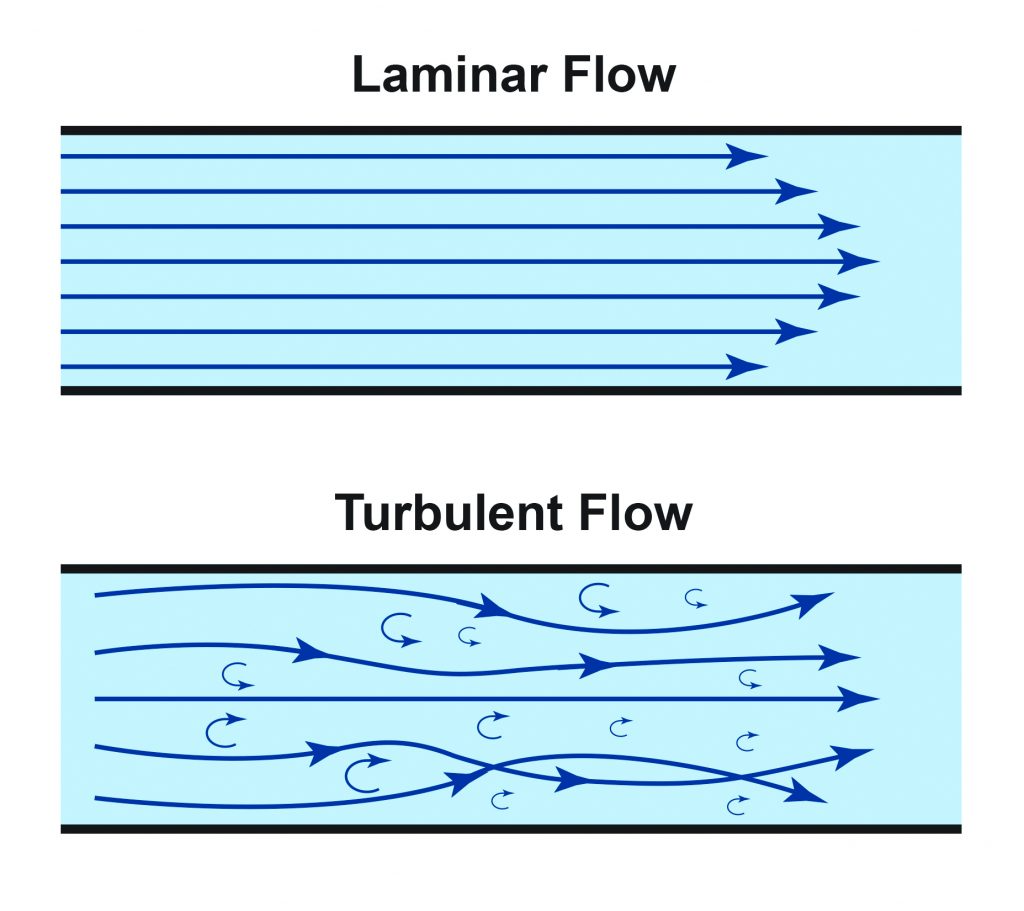
\includegraphics[width=.55\textwidth]{imagenes/imagenes18/T18IM15.png}
	\end{figure}
\end{multicols}


\section{Problemas}

\begin{prob}
¿Por qué los botes, cuando navegan próximos, sienten una fuerza que tiende a acercarlos? 	
\end{prob}

\begin{multicols}{2}
La sección entre los botes disminuye $\to$ aumenta la velocidad del fluido y disminuye la presión.
$$ \subrayado{\ \boldsymbol{ S\downarrow \quad v\uparrow \quad P\downarrow \ } \ }$$
Se crea un gradiente de presiones, $\ \overrightarrow{\grad}P \ $ desde las altas hacia las bajas presiones que da lugar a la aparición de una fuerza sobre cada bote que tiende a acercarlos.

Este fenómeno también se da en la carretera con coches/camiones.
\begin{figure}[H]
	\centering
	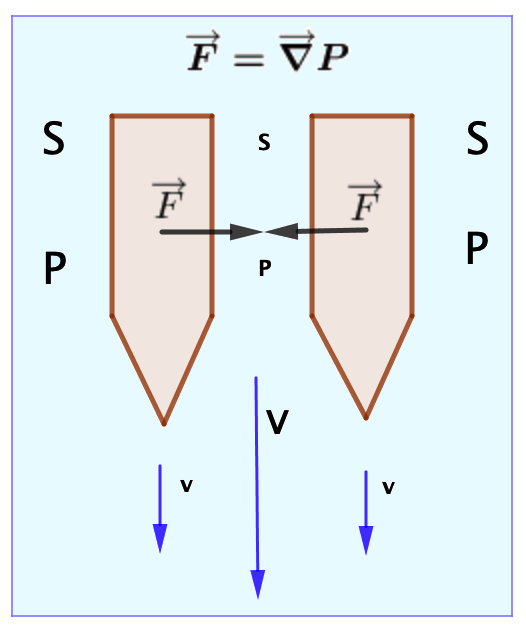
\includegraphics[width=.5\textwidth]{imagenes/imagenes18/T18IM16.png}
	\end{figure}	
\end{multicols}


\begin{prob}
a Un tanque lleno de agua hasta una altura $H$	 se le hace un agujero en una de sus paredes a una profundidad $h$ por debajo de la superficie de agua. $\ a)\ $ Encuentra la distancia $x$ del pie de la pared a la que el chorro de agua cae al suelo. $\ b)\ $ ¿Podría hacerse otro agujero a distinta profundidad de modo que el chorro tenga el mismo alcance que el el apartado anterior? $\ c) \ $ ¿A qué distancia debe practicarse el agujero para que el alcance del chorro sea máximo?
\end{prob}

\begin{multicols}{2}
--- a) $t=\dfrac{x}{\sqrt{2gh}};$

$H-h=\dfrac 1 2g t^2 = \dfrac {gx^2}{4gh} \ \to $

$x=\sqrt{4h(H-h}) \quad (*)$
\begin{figure}[H]
	\centering
	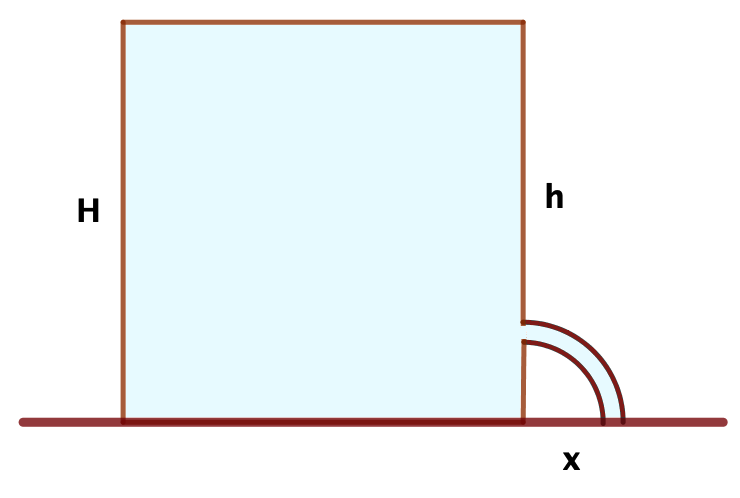
\includegraphics[width=.45\textwidth]{imagenes/imagenes18/T18IM17.png}
	\end{figure}	
\end{multicols}
--- b) Supongamos
$x_1=\sqrt{2gh_1}t_1;\ x_2=\sqrt{2gh_2}t_2 \ \to \ \sqrt{2gh_1}t_1= \sqrt{2gh_2}t_2$

$H-h_1=\dfrac 1 2 dt_1^2; \ H-h_2=\dfrac 1 2 dt_2^2 \ \to \ \dfrac{H-h_1}{H-h_2}=\dfrac{t_1^2}{t_2^2} \ \to \ t_2^2=\dfrac{H-h_2}{H-h_1}t_1^2$

$\sqrt{2dh_1}t_1=\sqrt{2dh_2}t_2 \sqrt{\dfrac{H-h_2}{H-h_1}} \ \to \ h_2=h_1 \dfrac{H-h_2}{H-h_1}$

$h_1-H-h_1^2=h_2(H-h_2) \ \to \ h_1^2-h_1H+h_2(H-h_2)=0$

$h_1=\dfrac{H\pm \sqrt{H^2-4h_2(H+h_2)}}{2}=\dfrac{H\pm} 2 h_2 - H{2} = \begin{cases} \ h_2\ \text{obvio} \\ \ H-h_2  \end{cases}$

Luego, $\ h_1=H-h_2$

--- c) De la ecuación $(*)$ del apartado $a)$, tenemos que $x=\sqrt{4h(H-h)}=\sqrt{4hH-4h^2}$, por lo que, para buscar el máximo derivaremos e igualaremos a cero:

$\displaystyle \dv{x}{t} =0=\dfrac{4H-8h}{2\sqrt{4hH-4h^2}} \ \to \ H-2h=0 \ \to h=\dfrac H 2$

\vspace{10mm} %****************************************
\begin{prob}
?`Con qué velocidad límite se elevará una burbuja de aire de $1\ \mathrm{mm}$ de diámetro en un líquido de $\eta=150\ \mathrm{centipoises}$ y densidad $\rho=0.90\ \mathrm{g\ cm}^{-3}$? ?`Cuál es esa velocidad límite en el agua?	
\end{prob}

$mg+f_{stokes}-E=0;\quad 6\pi r \eta v_L+\rho \dfrac 4 3 \pi r^3 g-\rho_0 \dfrac 4 3 \pi r^3 g=0$

$v_L=\dfrac 2 9 \dfrac{g r^2 (\rho_o-\rho)}{h} \approx \dfrac 2 9 \dfrac{gr^2 \rho_o}{h}$, puesto que $\rho << \rho_0$

--- a) $\rho_0=0.90\ \mathrm{g\ cm}^{-3};\ \eta=1.5 \ \mathrm{P} \quad \to \quad v_L=0.33 \mathrm{cm\ s}^{-1}$

--- b) $\rho_0=1\ \mathrm{g\ cm}^{-3};\ \eta=0.01 \ \mathrm{P} \quad \to \quad v_L=51.6 \mathrm{cm\ s}^{-1}$

\begin{prob}
Un líquido viscoso fluye en régimen laminar por la acción de la gravedad entre dos láminas verticales de gran superficie.

a) Si las láminas están separadas una distancia $2a$, pruébese que la velocidad del líquido a una distancia $x$ el plano mediador de las láminas viene dado por la ecuación $v=\dfrac{\rho g}{2 \eta}(a^2-x^2)$	

b) Dedúzcase la expresión del volumen de líquido que sale por unidad de tiempo por un área horizontal de anchura $L$ y espesor $2a$ (gasto).
\end{prob}
\begin{multicols}{2}
--- a) $\sum f_i=0 \to \dd m g+f_1-f_2=0$

$\displaystyle g\dd m +\eta A\dv{v}{x} + \eta A \dv{x} (v-\dd v)=0$

$\displaystyle d\dd m +\eta A \dd \left( \dv{v}{x} \right)=0$

$\displaystyle g \rho \cancel{A} \dd x + \eta \cancel{A} \dd \left( \dv{v}{x} \right)=0$

$\displaystyle g \rho  \dd x + \eta  \dv[2]{v}{x} \dd x=0$

$\displaystyle g \rho   + \eta  \dv[2]{v}{x}=0$
\begin{figure}[H]
	\centering
	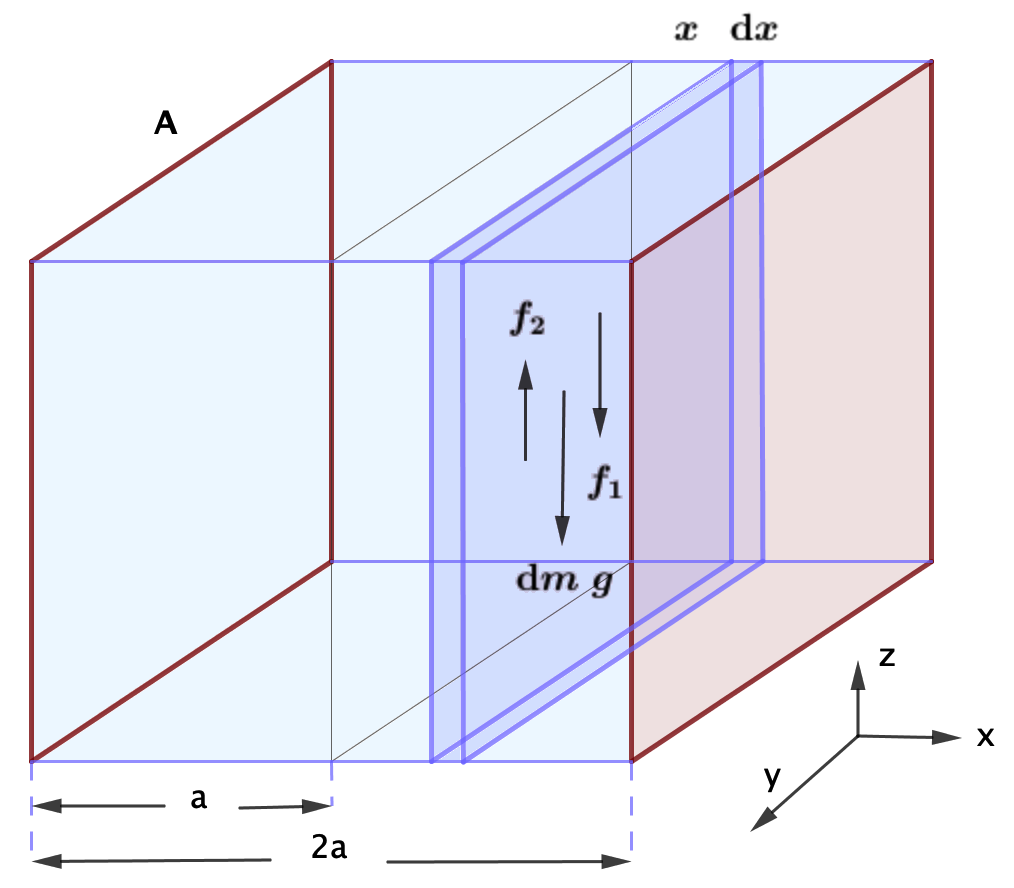
\includegraphics[width=.55\textwidth]{imagenes/imagenes18/T18IM18.png}
	\end{figure}	
\end{multicols}

$\displaystyle \dv[2]{v}{x}=-\dfrac{g\rho}{\eta}\ $  Ecuación diferencial de segundo orden que aún no se sabemos resolver y lo haremos de otro modo:

$\displaystyle \dv{x} \left( \dv{v}{x} \right) =\dv[2]{v}{x}=-\dfrac{g\rho}{\eta} \ \ \to \ \  \dd  \left( \dv{v}{x} \right) = -\dfrac{g\rho}{\eta} \dd x \ \ \to \ \  \dv{v}{x}=-\dfrac{g\rho}{\eta} x + \mathcal C$

$\displaystyle x=0 \to \left( \dv{v}{x} \right)_0=0 = -\dfrac{g\rho}{\eta} x + \mathcal C \ \to \  \mathcal C=0$

$\displaystyle \dv{v}{x}=-\dfrac{g\rho}{\eta} x \ \ \to \ \ \dd v = -\dfrac{g\rho}{\eta} x \dd x \ \ \to \ \ v=\dfrac{g \rho }{\eta}\dfrac{x^2}{2} +\mathcal B$

$x=a \to v_0 \to \mathcal B=-\dfrac{g \rho }{\eta}\dfrac{x^2}{2} \quad \Rightarrow \quad v\ =\ \dfrac{g\rho}{2\eta} \ (a^2-x^2)$

--- b) Gasto:  $\dd G=\displaystyle \dv{\dd \tau}{t}=\dv{t} (\dd \tau) = \dv{t} (L\dd x \dd y)=Lv\dd x + L \dd y \cancelto{0}{\dv{x}{t}}$

$\displaystyle \dd G= L v \dd x =L \dfrac{g\rho}{2\eta} (a^2-x^2) \dd x\ \ \to \ \ G=L \dfrac{g\rho}{2\eta} \int_{-a}^{+a} (x^2-a^2) \dd x$

$G\ =\ \dfrac 2 3 \ \dfrac{L \ g \ \rho}{\eta} \ a^3$
% ******************************************************
\newpage
\begin{myblock}{El efecto Venturi}

Consiste en un fenómeno en el que un fluido en movimiento dentro de un conducto cerrado disminuye su presión cuando aumenta la velocidad al pasar por una zona de sección menor.? En ciertas condiciones, cuando el aumento de velocidad es muy grande, se llegan a producir grandes diferencias de presión y entonces, si en este punto del conducto se introduce el extremo de otro conducto, se produce una aspiración del fluido de este conducto, que se mezclará con el que circula por el primer conducto. Este efecto, demostrado en 1797, recibe su nombre del físico italiano Giovanni Battista Venturi (1746-1822).

\begin{figure}[H]
	\centering
	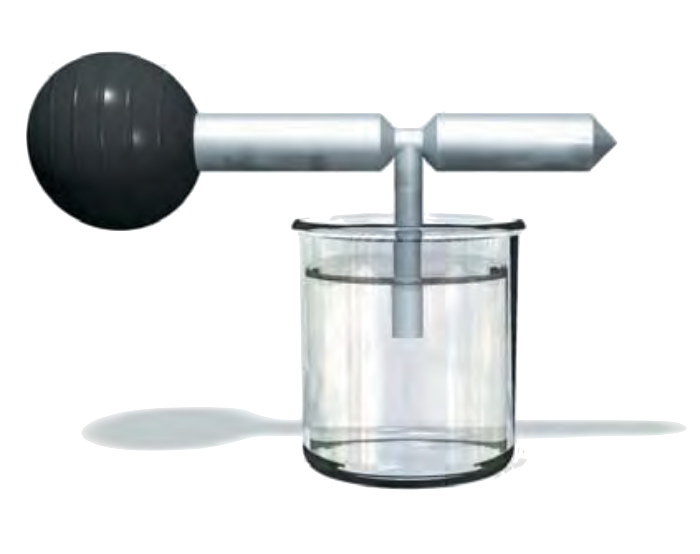
\includegraphics[width=.75\textwidth]{imagenes/imagenes18/T18IM10.png}
	\end{figure}

Una de las múltiples aplicaciones  del efecto Venturi la encontramos en el Pulverizador, un aparato empleado para rociar líquidos, consiste en pasar una corriente de aire a través de un tubo que tiene un estrangulamiento en el cual desemboca otro tubo, que vine de un recipiente lleno de líquido.	
\end{myblock}
